%----------------------------------------------------------------------------------------
%	KENAN FIRMANSYAH - BACKEND & SOFTWARE DEVELOPER VARIANT
%----------------------------------------------------------------------------------------

\documentclass[11pt,a4paper]{article}

\usepackage[utf8]{inputenc}
\usepackage[T1]{fontenc}
\usepackage{lmodern}
\usepackage[margin=0cm]{geometry}
\usepackage{hyperref}
\usepackage{fontawesome5}
\usepackage{xcolor}
\usepackage{tikz}
\usepackage{graphicx}
\usepackage{enumitem}
\usepackage{parskip}
\usepackage{multicol}
\usepackage{fancyhdr}
\usepackage{calc}

\definecolor{sidebar}{RGB}{245, 245, 245}
\definecolor{mainbg}{RGB}{255, 255, 255}
\definecolor{accent}{RGB}{180, 150, 100}
\definecolor{darktext}{RGB}{40, 40, 40}
\definecolor{lighttext}{RGB}{100, 100, 100}

\hypersetup{
    colorlinks=true,
    linkcolor=darktext,
    urlcolor=accent,
    pdftitle={Kenan Firmansyah - Backend Developer Resume},
    pdfauthor={Kenan Firmansyah}
}

\pagestyle{empty}
\setlength{\parindent}{0pt}

\newcommand{\sidesection}[1]{%
    {\large\bfseries\MakeUppercase{#1}}\\[6pt]%
}

\newcommand{\mainsection}[1]{%
    {\large\bfseries\MakeUppercase{#1}}\\[8pt]%
}

\newcommand{\jobentry}[2]{%
    \textbf{#1}\\
    {\small\color{lighttext}#2}\\[4pt]%
}

\begin{document}

\begin{tikzpicture}[remember picture, overlay]
    \fill[sidebar] (current page.north west) rectangle ([xshift=6.5cm]current page.south west);
    \fill[mainbg] ([xshift=6.5cm]current page.north west) rectangle (current page.south east);
    \fill[accent] ([xshift=6.5cm, yshift=-1cm]current page.north west) rectangle ([yshift=-1.05cm]current page.north east);
\end{tikzpicture}

\begin{minipage}[t]{6cm}
\vspace{0.8cm}
\hspace{0.5cm}
\begin{minipage}[t]{5.5cm}

\begin{center}
\begin{tikzpicture}
    \clip (0,0) rectangle (4.5cm, 4.5cm);
    \node[anchor=center] at (2.25cm, 2.25cm) {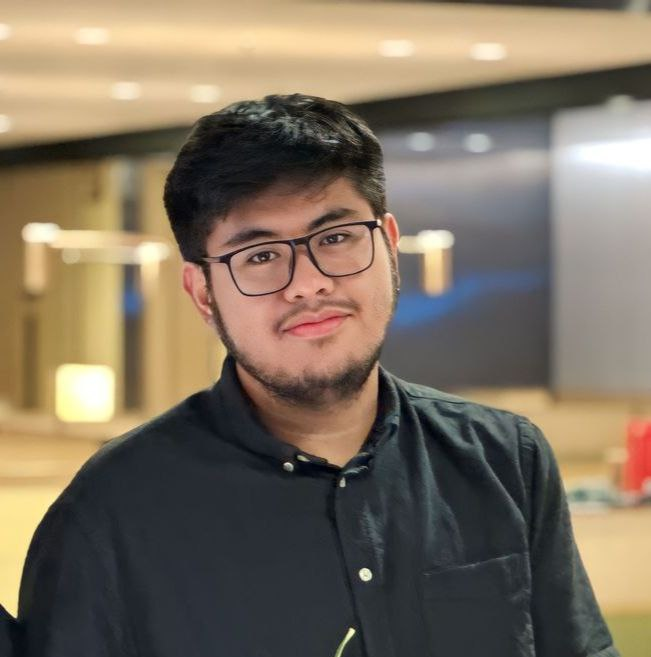
\includegraphics[width=4.5cm]{CV_ProfilePic.jpg}};
\end{tikzpicture}
\end{center}

\vspace{0.8cm}

\sidesection{Education}

\textbf{Bachelor of Computer Engineering, Major in Game Technology}\\[4pt]
{\small Electronic Engineering Polytechnic Institute of Surabaya (2020 - 2024)\\
GPA 3.67 (Cumlaude)}

\vspace{0.6cm}

\sidesection{Tech Stack}

{\small\textbf{Languages}}
\begin{itemize}[leftmargin=*, nosep, itemsep=2pt]
    \item C++, Python, JavaScript (Node.js)
\end{itemize}

\vspace{0.2cm}

{\small\textbf{Backend \& Data}}
\begin{itemize}[leftmargin=*, nosep, itemsep=2pt]
    \item Node.js, Redis, Jupyter Notebook
\end{itemize}

\vspace{0.2cm}

{\small\textbf{DevOps \& Infrastructure}}
\begin{itemize}[leftmargin=*, nosep, itemsep=2pt]
    \item Docker, Dokploy, Proxmox, Linux
\end{itemize}

\vspace{0.2cm}

{\small\textbf{Engines}}
\begin{itemize}[leftmargin=*, nosep, itemsep=2pt]
    \item Unity (C\#), Unreal (C++ / Blueprint)
\end{itemize}

\vspace{0.8cm}

\sidesection{Contact}

\faIcon{linkedin} \href{https://linkedin.com/in/kenanfirmansyah}{Kenan Firmansyah}\\[6pt]
\faIcon{github} \href{https://github.com/Kenanfir}{Kenanfir}\\[6pt]
\faIcon{globe} \href{https://nandev.dev}{nandev.dev}\\[6pt]
\faIcon{phone} +6285175447540\\[6pt]
\faIcon{envelope} realkenanfir@gmail.com\\[10pt]

{\small\color{lighttext}Kalijudan, Mulyorejo, Surabaya, Jawa Timur 60114}\\[6pt]

{\small\color{lighttext}Holland Village Jakarta, Cemp. Putih, Jakarta Pusat, DKI Jakarta 10510}

\end{minipage}
\end{minipage}%
%
\begin{minipage}[t]{14cm}
\vspace{0.5cm}
\hspace{0.8cm}
\begin{minipage}[t]{12.5cm}

{\Huge\bfseries\MakeUppercase{Kenan Firmansyah}}\\[6pt]
{\large\bfseries BACKEND \& SOFTWARE DEVELOPER}\\[12pt]

{\small Software developer with experience across backend services, self-hosted infrastructure, and data engineering. Comfortable across the stack from Node.js services and Redis-backed systems to Proxmox/Docker hypervisor work, with a research background applying Python and ML to production problems.}

\vspace{0.5cm}

\mainsection{Experience}

\jobentry{Game Developer}{Agate | 2026 Feb - 2026 May}
\begin{itemize}[leftmargin=*, nosep, itemsep=2pt, topsep=2pt]
    \item Software engineering on an unannounced commercial project at one of Indonesia's largest game studios.
\end{itemize}

\vspace{0.3cm}

\jobentry{Apple Developer Academy @ BINUS (Alum)}{2025 Feb - 2025 Dec, Bali}
\begin{itemize}[leftmargin=*, nosep, itemsep=2pt, topsep=2pt]
    \item 10-month intensive in product engineering: API design, networking, prototyping, iterative testing in interdisciplinary teams.
\end{itemize}

\vspace{0.3cm}

\jobentry{Lead Developer (Unreal Engine, C++)}{Starpixel Studios | 2024 Oct - 2025 April}
\begin{itemize}[leftmargin=*, nosep, itemsep=2pt, topsep=2pt]
    \item Designed and shipped multiplayer networking systems for a real-time horror title.
    \item Wrote C++ for performance-critical paths; managed build, bug-tracking, and internal docs.
\end{itemize}

\vspace{0.3cm}

\jobentry{Data Scientist (Intern)}{PT. eBdesk | 2023, 6 months}
\begin{itemize}[leftmargin=*, nosep, itemsep=2pt, topsep=2pt]
    \item Built Python data pipelines for scraping, analysis, and visualization (Selenium, Gephi, Tableau, Jupyter).
\end{itemize}

\end{minipage}
\end{minipage}

\newpage

\begin{tikzpicture}[remember picture, overlay]
    \fill[accent] (current page.north west) rectangle ([yshift=-0.8cm]current page.north east);
\end{tikzpicture}

\vspace{1.2cm}

\begin{center}
{\large\bfseries\MakeUppercase{Selected Projects \& Additional Work}}
\end{center}

\vspace{0.5cm}

\hspace{1cm}
\begin{minipage}[t]{18cm}

\begin{minipage}[t]{0.8cm}
{\Large\bfseries 1}
\end{minipage}%
\begin{minipage}[t]{17cm}
{\large\bfseries BACKEND, INFRASTRUCTURE \& TOOLING}\\[8pt]

\textbf{Home Server (Personal Infrastructure)}\\
{\small 2023 Oct - 2023 Dec \textbar{} Proxmox, Docker, Linux}
\begin{itemize}[leftmargin=*, nosep, itemsep=2pt, topsep=2pt]
    \item Designed and operated a multi-purpose self-hosted server: NAS, database server, and compute node.
    \item Proxmox-based virtualization with Linux guests; containerized services via Docker.
\end{itemize}

\vspace{0.3cm}

\textbf{Findect — iOS Backend Developer}\\
{\small Apple Developer Academy cohort project | 2025 \textbar{} Team of 6}
\begin{itemize}[leftmargin=*, nosep, itemsep=2pt, topsep=2pt]
    \item Built backend services for an LLM-powered professional networking app; matching and discovery layer.
\end{itemize}

\vspace{0.3cm}

\textbf{Agreely — Software House \& Freelance Platform (On-going)}\\
{\small Web / App stack, team of 3}
\begin{itemize}[leftmargin=*, nosep, itemsep=2pt, topsep=2pt]
    \item Founding contributor on a freelance-marketplace platform; covers full-stack engineering and ops.
\end{itemize}

\vspace{0.3cm}

\textbf{Paid — Sport Split Bill}\\
{\small Apple Developer Academy cohort project | 2025 \textbar{} 8+ weeks, team of 3}
\begin{itemize}[leftmargin=*, nosep, itemsep=2pt, topsep=2pt]
    \item Organizer-side cost \& payment manager for recurring group activities; backend logic for splitting, tracking, and reconciliation.
\end{itemize}

\end{minipage}

\vspace{0.6cm}

\begin{minipage}[t]{0.8cm}
{\Large\bfseries 2}
\end{minipage}%
\begin{minipage}[t]{17cm}
{\large\bfseries APPLIED RESEARCH \& DATA}\\[8pt]

\textbf{Five peer-reviewed publications} in IEEE Access, IJIES, ICVR, and TCCE on adaptive systems, reinforcement learning (Q-Learning + fuzzy logic), and context-aware recommender systems. Built on Python, Jupyter, and engine-side C++ for evaluation harnesses. \emph{F1 up to 0.71; +35\% session length} on the DDA paper.

\end{minipage}

\vspace{0.5cm}

\begin{minipage}[t]{0.8cm}
{\Large\bfseries 3}
\end{minipage}%
\begin{minipage}[t]{17cm}
{\large\bfseries SHIPPED SOFTWARE \& GAMES}\\[8pt]

\textbf{Saturated} (Mac App Store, Apple Silicon) — Programmer \& Project Manager, JoyBait Studio.\\
\textbf{Milky Ice Jump} (iOS App Store) — Freelance iOS port + ad integration.\\
\textbf{Xanthous} (Thesis, EEPIS) — AI-driven VR horror in Unreal, 2023-2024.\\
\textbf{9+ Game Jams} across Unity, Unreal, and multiplayer stacks (Photon networking) — recurring roles as gameplay programmer, AI programmer, and solo dev.

\end{minipage}

\vspace{0.8cm}

\begin{center}
\href{https://nandev.dev}{\bfseries\color{accent}\underline{View More...}}\\[4pt]
{\small nandev.dev}
\end{center}

\end{minipage}

\end{document}
